\chapter{ĐỀ XUẤT VÀ BÁO CÁO ĐỀ TÀI THỰC TẬP}
\textbf{\textit{Cần có phần tóm tắt mỗi khi bắt đầu chương}}\textit{Chương 2 trình bày tổng quan toàn diện về một số kỹ thuật thường được sử dụng, cũng như một số kỹ thuật khớp tên được phát triển gần đây như nghiên cứu các phương pháp tiếp cận vấn đề đối sánh tên chứng minh độ chính xác bằng cách kết hợp phương pháp tương tự cơ sở ký tự và phương pháp học sâu, phương pháp Name2Vec để giải quyết việc đối sánh tên bằng cách sử dụng mô hình học sâu để tìm hiểu ngữ nghĩa phù hợp với tên bằng cách sử dụng tổ hợp của Name2Vec dựa trên ký tự và các chỉ số tương đồng của hai chuỗi.}.

Phần này sinh viên mô tả sơ lược về hệ thống cần xây dựng, lý do tại sao lại chọn đề tài đó  đó, ý nghĩa/tầm quan trọng của đề tài với thực tiễn nghiên cứu và ứng dụng.

Tiêu đề của chương này có thể để là ``đặt vấn đề'', hoặc lấy chính tên của Hệ thống mà sinh viên định xây dựng, ví dụ có thể đặt tiêu đề là ``Hệ thống abc …” 
\section{Giới thiệu chung về đề tài}
\subsection*{Các giải pháp hiện tại và hạn chế}
\label{sec:giaiphap}
Sinh viên trước tiên cần trình bày tổng quan các công nghệ xây dựng cho hệ thống đó hiện nay cho hệ thống giới thiệu ở phần \ref{sec:dvd}. Sau đấy, sinh viên đưa ra các xu hướng của các giải pháp kỹ thuật hiện tại. 

\subsection*{Mục tiêu và định hướng giải pháp}
Trong chương này, sinh viên trước hết trình bày mục tiêu của Bài tập lớn là gì, sau đấy sinh viên đề xuất định hướng giải pháp xây dựng hệ thống của mình. Tốt nhất là với trình bày từng phương pháp đối với mỗi vấn đề nêu ra trong chương \ref{sec:giaiphap}. 
\begin{figure}[h]
\centering
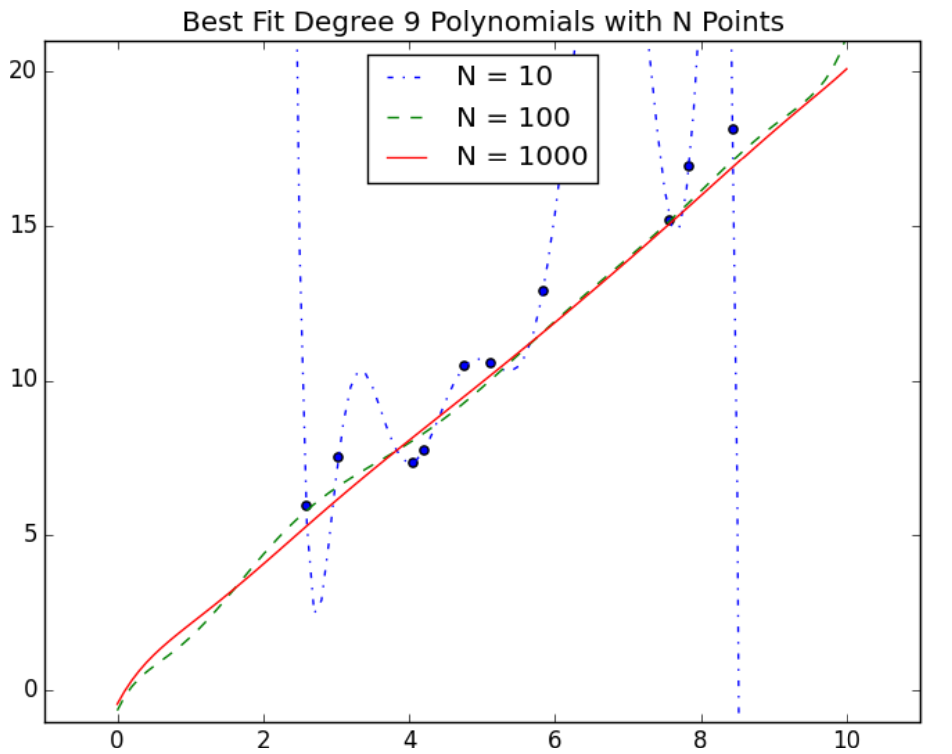
\includegraphics[width=0.5\linewidth]{Figures/bias.png}
\caption{Internet vạn vật}
\label{fig:iot}
\end{figure}

\subsection*{Đóng góp của tài}
Trong phần này sinh viên liệt kê cụ thể, ngắn gọn các đóng góp của bài tập lớn. Ví dụ: 

Bài tập lớn này có 3 đóng góp chính như sau:

\begin{enumerate}
\item Bài tập lớn này đưa ra các khảo sát công nghệ về xây dựng hệ thống ABC
\item Đưa ra hương pháp thực hiện, các bước tiến hành cài đặt hệ thống ABC
\item \ldots 
\end{enumerate}
Ví dụ tham khảo mô tả chương trong phần bố cục đồ án tốt nghiệp: Chương *** trình bày đóng góp chính của đồ án, đó là một nền tảng ABC cho phép khai phá và tích hợp nhiều nguồn dữ liệu, trong đó mỗi nguồn dữ liệu lại có định dạng đặc thù riêng. Nền tảng ABC được phát triển dựa trên khái niệm DEF, là các module ngữ nghĩa trợ giúp người dùng tìm kiếm, tích hợp và hiển thị trực quan dữ liệu theo mô hình cộng tác và mô hình phân tán.  

\subsection*{Giới thiệu về bài toán xử lý ảnh}

\subsection*{Giới thiệu về Deep learning}

\subection{Đánh giá mô hình Deep learning}

\section{Cơ sở lý thuyết và các nghiên cứu liên quan}
\subsection*{Tổng quan hệ thống nhận diện khuôn mặt}
Một hệ thống nhận diện khuôn mặt gồm nhiều phần để từ đó xây dựng nên một hệ thống nhận diện khuôn mặt hoàn chỉnh. Trong đồ án này sẽ khảo sát các thành phần của hệ thống nhận diện khuôn mặt gồm 5 phần chính:
\begin{figure}[h]
\centering
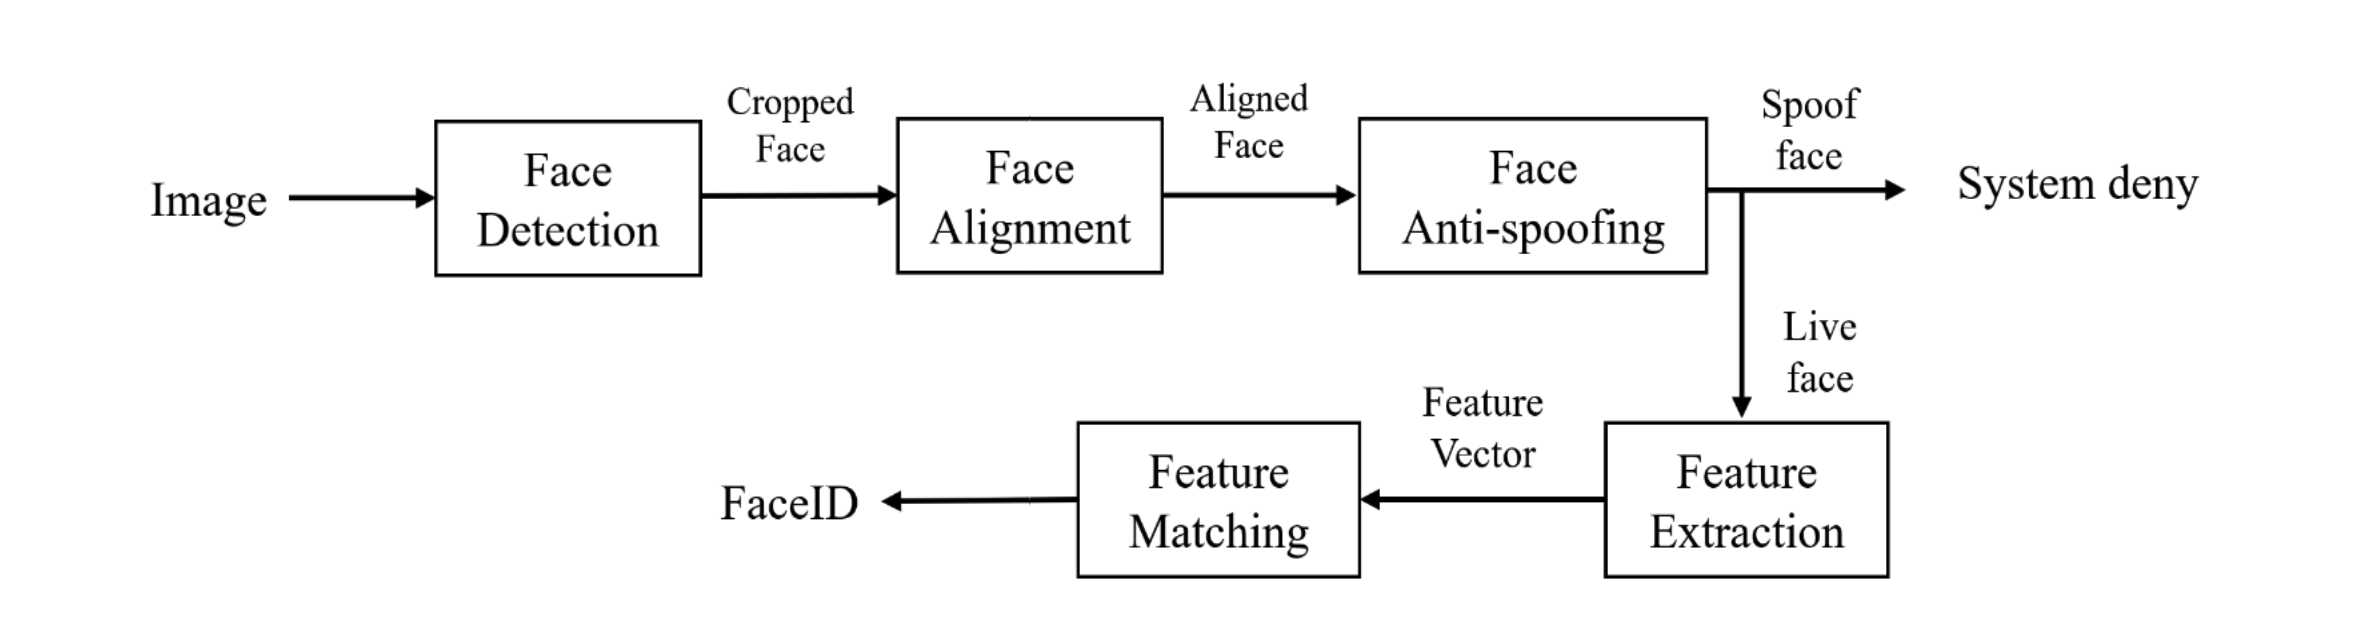
\includegraphics[width=1.1\linewidth]{Figures/LuongMohinh}
\caption{Internet vạn vật}
\label{fig:iot}
\end{figure}
\begin{itemize}
    \item Bộ phát hiện khuôn mặt (\textit{Face Detection}): Xác định vị trí khuôn mặt trong toàn bộ bức ảnh.
    
     \item Bộ căn chỉnh khuôn mặt (\textit{Face Alignment}): Xác định các điểm mốc trên khuôn mặt (facial landmark detector) sau đó chuẩn hóa, căn chỉnh lại khuôn mặt được phát hiện trong bộ phát hiện khuôn mặt trước đó.
     
      \item Bộ phát hiện chống giả mạo (\textit{Face Anti-spoofing}): Kiểm tra khuôn mặt của người dùng hệ thống là khuôn mặt thật hay khuôn mặt giả.
       \item Bộ trích xuất đặc trưng khuôn mặt (\textit{Feature Extraction}): Mã hóa, trích xuất các thông tin có trên gương mặt của ảnh đầu vào thành một vector đặc trưng đại diện cho khuôn mặt đó.
       
        \item Bộ nhận diện khuôn mặt (\textit{Face Matching}): Tìm kiếm vector đặc trưng của khuôn mặt đại diện cho ai trong hệ thống. 
\end{itemize}
\subsubsection*{Bộ phát hiện khuôn mặt}
\subsubsection*{Bộ căn chỉnh khuôn mặt}
\subsubsection*{Bộ phát hiện chống giả mạo}
\subsubsection*{Bộ trích xuất đặc trưng khuôn mặt}
\subsubsection*{Bộ nhận diện khuôn mặt}

\subsection*{Mô hình InceptionResnetV2}

Trình bày khái quát về đề tài bao gồm lý do và động lực chọn đề tài là gì? Khảo sát về công nghệ thực hiện hoặc sử dụng thống kê hay lý do kỹ thuật để thấy được việc lựa chọn là đúng đắn.


Phần này sinh viên mô tả sơ lược về hệ thống cần xây dựng, lý do tại sao lại chọn đề tài đó  đó, ý nghĩa/tầm quan trọng của đề tài với thực tiễn nghiên cứu và ứng dụng.

Tiêu đề của chương này có thể để là ``đặt vấn đề'', hoặc lấy chính tên của Hệ thống mà sinh viên định xây dựng, ví dụ có thể đặt tiêu đề là ``Hệ thống abc …” 


\subsection*{Giới thiệu công cụ gán nhãn dữ liệu mã nguồn mở LabelImg}
Sinh viên trước tiên cần trình bày tổng quan các công nghệ xây dựng cho hệ thống đó hiện nay cho hệ thống giới thiệu ở phần \ref{sec:dvd}. Sau đấy, sinh viên đưa ra các xu hướng của các giải pháp kỹ thuật hiện tại. 
\subsection*{Tìm hiểu OCR}
\subsection*{Tìm hiểu Web framework Flask}


\section{XÂY DỰNG CHƯƠNG TRÌNH}
\textbf{\textit{Cần có phần tóm tắt mỗi khi bắt đầu chương}}\textit{Chương 2 trình bày tổng quan toàn diện về một số kỹ thuật thường được sử dụng, cũng như một số kỹ thuật khớp tên được phát triển gần đây như nghiên cứu các phương pháp tiếp cận vấn đề đối sánh tên chứng minh độ chính xác bằng cách kết hợp phương pháp tương tự cơ sở ký tự và phương pháp học sâu, phương pháp Name2Vec để giải quyết việc đối sánh tên bằng cách sử dụng mô hình học sâu để tìm hiểu ngữ nghĩa phù hợp với tên bằng cách sử dụng tổ hợp của Name2Vec dựa trên ký tự và các chỉ số tương đồng của hai chuỗi.}.

\subsection*{Sơ đồ hệ thống}
Một hệ thống nhận diện khuôn mặt gồm nhiều phần để từ đó xây dựng nên một hệ thống nhận diện khuôn mặt hoàn chỉnh. Trong đồ án này sẽ khảo sát các thành phần của hệ thống nhận diện khuôn mặt gồm 5 phần chính:
\begin{figure}[h]
\centering
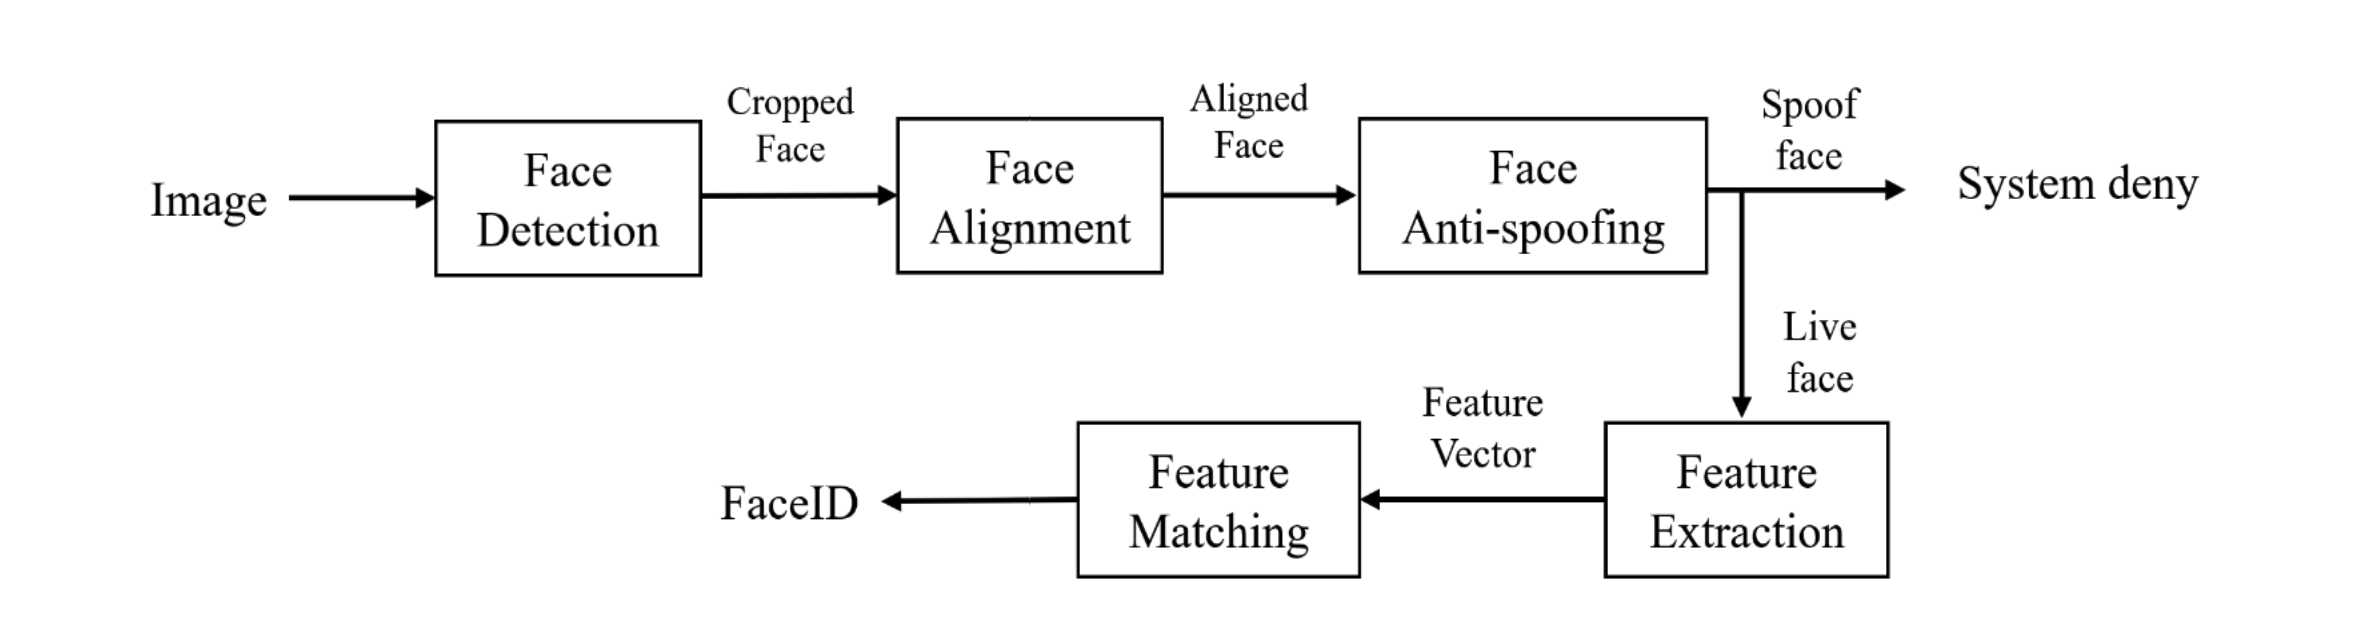
\includegraphics[width=1.1\linewidth]{Figures/LuongMohinh}
\caption{Internet vạn vật}
\label{fig:iot}
\end{figure}

\subsection*{Các bước thực hiện}
\subsubsection*{Thu thập dữ liệu}
\subsubsection*{Gán nhãn dữ liệu}
\subsubsection*{Tiền xử lý dữ liệu}
\subsubsection*{Cài đặt mô hình dự đoán}
\subsubsection*{Đánh giá mô hình dự đoán}
\subsection*{Xây dựng Website demo}
\subsubsection*{Phân tích hệ thống}
\textbf{Mô tả các chức năng chính của hệ thống:}

Hệ thống điểm danh bằng khuôn mặt sẽ gồm 3 actor chính: Admin, Giảng viên, Sinh
viên. Các chức năng chính của các actor sau khi đăng nhập vào hệ thống:

\section*{Kết luận chương}
Trong phần Kết chương, sinh viên đưa ra một số kết luận quan trọng của chương. Những vấn đề mở ra trong Tổng quan cần được tóm tắt lại nội dung và cách giải quyết/thực hiện như thế nào. Sinh viên lưu ý không viết Kết chương giống hệt Tổng quan. Sau khi đọc phần Kết chương, người đọc sẽ nắm được sơ bộ nội dung và giải pháp cho các vấn đề đã trình bày trong chương. Trong Kết chương, Sinh viên nên có thêm câu liên kết tới chương tiếp theo.

Ví dụ về phần Kết chương: Chương này đã phân tích chi tiết sáu nhóm công cụ tích hợp dữ liệu. Nhóm công cụ ABC và DEF thích hợp với những bài toán tích hợp dữ liệu phạm vi nhỏ. Trong khi đó, nhóm công cụ GHK lại chứng tỏ thế mạnh của mình với những bài toán cần độ chính xác cao, v.v. Từ kết quả nghiên cứu và phân tích về sáu nhóm công cụ tích hợp dữ liệu này, tôi đã thực hiện phát triển phần mềm tự động bóc tách và tích hợp dữ liệu sử dụng nhóm công cụ GHK. Phần này được trình bày trong chương tiếp theo – Chương 5.


% Khôi phục lại margin


% Khôi phục lại margin

